\documentclass{article}

% Short communications of approximately 3000 words are also accepted. 
% These papers should contain no more than two figures, two tables, and thirty references. 
% A short abstract of fewer than 200 words is acceptable.

% Bibliography
\usepackage{natbib}
\bibpunct{(}{)}{;}{a}{}{;}

\usepackage[english]{babel}

% Use 'It was found that something is something (Name 1234)' style
\setcitestyle{authoryear,open={},close={}}

% Affiliations
\usepackage{authblk}
\title{The error when inferring phylogenies with incipient species by a Birth-Death model}
% \subtitle{Should protracted speciation be incorporated in phylogenetic tree construction methods?}

\author[1]{Rich\`el J.C. Bilderbeek}
\author[1]{Rampal S. Etienne}
\affil[1]{Groningen Institute for Evolutionary Life Sciences, University of Groningen, Groningen, The Netherlands}

% Use double spacing
\usepackage{setspace}
\doublespacing

\usepackage{listings}
\usepackage{hyperref}
\usepackage{todonotes}
\usepackage{verbatim}
\usepackage{pgf}
\usepackage{bm}

% TikZ and friends
\usepackage{tikz}
\usepackage{tkz-graph}
\usepackage{pgf}
\usetikzlibrary{arrows,automata}

% Style of listings
% From http://r.789695.n4.nabble.com/How-to-nicely-display-R-code-with-the-LaTeX-package-listings-tp4648110.html
\usepackage{fancyvrb} 
\definecolor{codegreen}{rgb}{0,0.6,0}
\definecolor{codegray}{rgb}{0.5,0.5,0.5}
\definecolor{codepurple}{rgb}{0.58,0,0.82}
\definecolor{backcolor}{rgb}{0.95,0.95,0.92}
\lstdefinestyle{mystyle}{
  language=R,% set programming language
  basicstyle=\ttfamily\small,% basic font style
  commentstyle=\color{gray},% comment style
  % numbers=left,% display line numbers on the left side
  numberstyle=\scriptsize,% use small line numbers
  numbersep=10pt,% space between line numbers and code
  tabsize=2,% sizes of tabs
  showstringspaces=false,% do not replace spaces in strings by a certain character
  captionpos=b,% positioning of the caption below
  breaklines=true,% automatic line breaking
  escapeinside={(*}{*)},% escaping to LaTeX
  fancyvrb=true,% verbatim code is typset by listings
  extendedchars=false,% prohibit extended chars (chars of codes 128--255)
  alsoletter={.<-},% becomes a letter
  alsoother={$},% becomes other
  otherkeywords={!=, ~, $, \&, \%/\%, \%*\%, \%\%, <-, <<-, /},% other keywords
  deletekeywords={c}% remove keywords 
}
\lstset{style=mystyle}

% Adds numbered lines
\usepackage{lineno}
\linenumbers

\begin{document}

\maketitle

%%%%%%%%%%%%%%%%%%%%%%%%%%%%%%%%%%%%%%%%%%%%%%%%%%%%%%%%%%%%%%%%%%%%%%%%%%%%%%%%
% Create the TikZ picture for fig:experiment, for only 'youngest'
%%%%%%%%%%%%%%%%%%%%%%%%%%%%%%%%%%%%%%%%%%%%%%%%%%%%%%%%%%%%%%%%%%%%%%%%%%%%%%%%
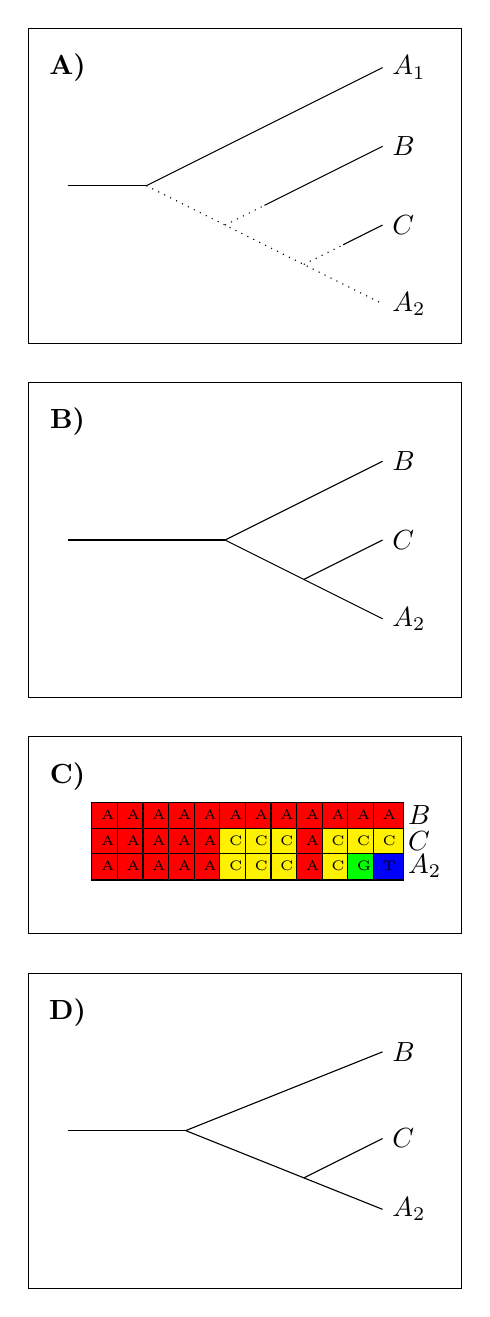
\begin{tikzpicture}[scale = 0.5]

  % Incipient species tree
  \begin{scope}[shift={(0,0)}] 

    \node[font = \bf] at (0, 0) {A)};
    \draw (-1,1) rectangle (10,-7);

    % Drawing of the phylogeny
    \begin{scope}[shift={(0,-3)}] 
      \draw (0, 0) -- (2,  0); % stem 
      \draw (2, 0) -- (8,  3) node[anchor=west] {$A_1$};
      \draw[dotted] (4,  -1) -- (5, -0.5); \draw (5, -0.5) -- (8, 1) node[anchor=west] {$B$};
      \draw[dotted] (6,  -2) -- (7, -1.5); \draw (7, -1.5) -- (8, -1) node[anchor=west] {$C$};
      \draw[dotted] (2,0) -- (8, -3) node[anchor=west] {$A_2$};
    \end{scope} % Drawing of the phylogeny

  \end{scope}

  % Species tree, youngest
  \begin{scope}[shift={( 0,-9)}] 

    \node[font = \bf] at (0, 0) {B)};
    \draw (-1,1) rectangle (10,-7);

    % Drawing of the species tree, youngest
    \begin{scope}[shift={(0,-3)}] 
      \draw (0, 0) -- (4,  0); % stem 
      \draw (4, 0) -- (8,  2) node[anchor=west] {$B$};
      \draw (6,-1) -- (8,  0) node[anchor=west] {$C$};
      \draw (4, 0) -- (8, -2) node[anchor=west] {$A_2$};
    \end{scope} % Drawing of the species tree, youngest

  \end{scope}

  % Alignment, youngest
  \begin{scope}[shift={(0,-18)}] 

    \node[font = \bf] at (0.0, 0  ) {C)};
    \draw (-1,1) rectangle (10,-4);

    % Drawing of the alignment
    \begin{scope}[shift={(1,-1)}, text width = 1.5mm, text height = 1.0mm, align = center, scale = 1.3] 

      \node[draw, fill = red   ] at (0.0, 0  ) {\tiny A};
      \node[draw, fill = red   ] at (0.5, 0  ) {\tiny A};
      \node[draw, fill = red   ] at (1.0, 0  ) {\tiny A};
      \node[draw, fill = red   ] at (1.5, 0  ) {\tiny A};
      \node[draw, fill = red   ] at (2.0, 0  ) {\tiny A};
      \node[draw, fill = red   ] at (2.5, 0  ) {\tiny A};
      \node[draw, fill = red   ] at (3.0, 0  ) {\tiny A};
      \node[draw, fill = red   ] at (3.5, 0  ) {\tiny A};
      \node[draw, fill = red   ] at (4.0, 0  ) {\tiny A};
      \node[draw, fill = red   ] at (4.5, 0  ) {\tiny A};
      \node[draw, fill = red   ] at (5.0, 0  ) {\tiny A};
      \node[draw, fill = red   ] at (5.5, 0  ) {\tiny A};
      \node[                   ] at (6.0, -0.1) {$B$};

      \node[draw, fill = red   ] at (0.0, -0.5) {\tiny A};
      \node[draw, fill = red   ] at (0.5, -0.5) {\tiny A};
      \node[draw, fill = red   ] at (1.0, -0.5) {\tiny A};
      \node[draw, fill = red   ] at (1.5, -0.5) {\tiny A};
      \node[draw, fill = red   ] at (2.0, -0.5) {\tiny A};
      \node[draw, fill = yellow] at (2.5, -0.5) {\tiny C};
      \node[draw, fill = yellow] at (3.0, -0.5) {\tiny C};
      \node[draw, fill = yellow] at (3.5, -0.5) {\tiny C};
      \node[draw, fill = red   ] at (4.0, -0.5) {\tiny A};
      \node[draw, fill = yellow] at (4.5, -0.5) {\tiny C};
      \node[draw, fill = yellow] at (5.0, -0.5) {\tiny C};
      \node[draw, fill = yellow] at (5.5, -0.5) {\tiny C};
      \node[                   ] at (6.0, -0.6) {$C$};

      \node[draw, fill = red   ] at (0.0, -1.0) {\tiny A};
      \node[draw, fill = red   ] at (0.5, -1.0) {\tiny A};
      \node[draw, fill = red   ] at (1.0, -1.0) {\tiny A};
      \node[draw, fill = red   ] at (1.5, -1.0) {\tiny A};
      \node[draw, fill = red   ] at (2.0, -1.0) {\tiny A};
      \node[draw, fill = yellow] at (2.5, -1.0) {\tiny C};
      \node[draw, fill = yellow] at (3.0, -1.0) {\tiny C};
      \node[draw, fill = yellow] at (3.5, -1.0) {\tiny C};
      \node[draw, fill = red   ] at (4.0, -1.0) {\tiny A};
      \node[draw, fill = yellow] at (4.5, -1.0) {\tiny C};
      \node[draw, fill = green ] at (5.0, -1.0) {\tiny G};
      \node[draw, fill = blue  ] at (5.5, -1.0) {\tiny T};
      \node[                   ] at (6.0, -1.1) {$A_2$};

    \end{scope} % Drawing of the alignment

  \end{scope}

  % Estimated species tree, youngest
  \begin{scope}[shift={(0,-24)}] 

    \node[font = \bf] at (0, 0) {D)};
    \draw (-1,1) rectangle (10,-7);

    \begin{scope}[shift={(0,-3)}] 
      \draw (0, 0) -- (3,  0);
      \draw (3, 0) -- (8,  2) node[anchor=west] {$B$};
      \draw (6,-1.2) -- (8, -0.2) node[anchor=west] {$C$};
      \draw (3, 0) -- (8, -2) node[anchor=west] {$A_2$};
    \end{scope}

  \end{scope}

\end{tikzpicture}
%%%%%%%%%%%%%%%%%%%%%%%%%%%%%%%%%%%%%%%%%%%%%%%%%%%%%%%%%%%%%%%%%%%%%%%%%%%%%%%%


%%%%%%%%%%%%%%%%%%%%%%%%%%%%%%%%%%%%%%%%%%%%%%%%%%%%%%%%%%%%%%%%%%%%%%%%%%%%%%%%
% Create the TikZ picture for fig:experiment, both sampling methods
%%%%%%%%%%%%%%%%%%%%%%%%%%%%%%%%%%%%%%%%%%%%%%%%%%%%%%%%%%%%%%%%%%%%%%%%%%%%%%%%
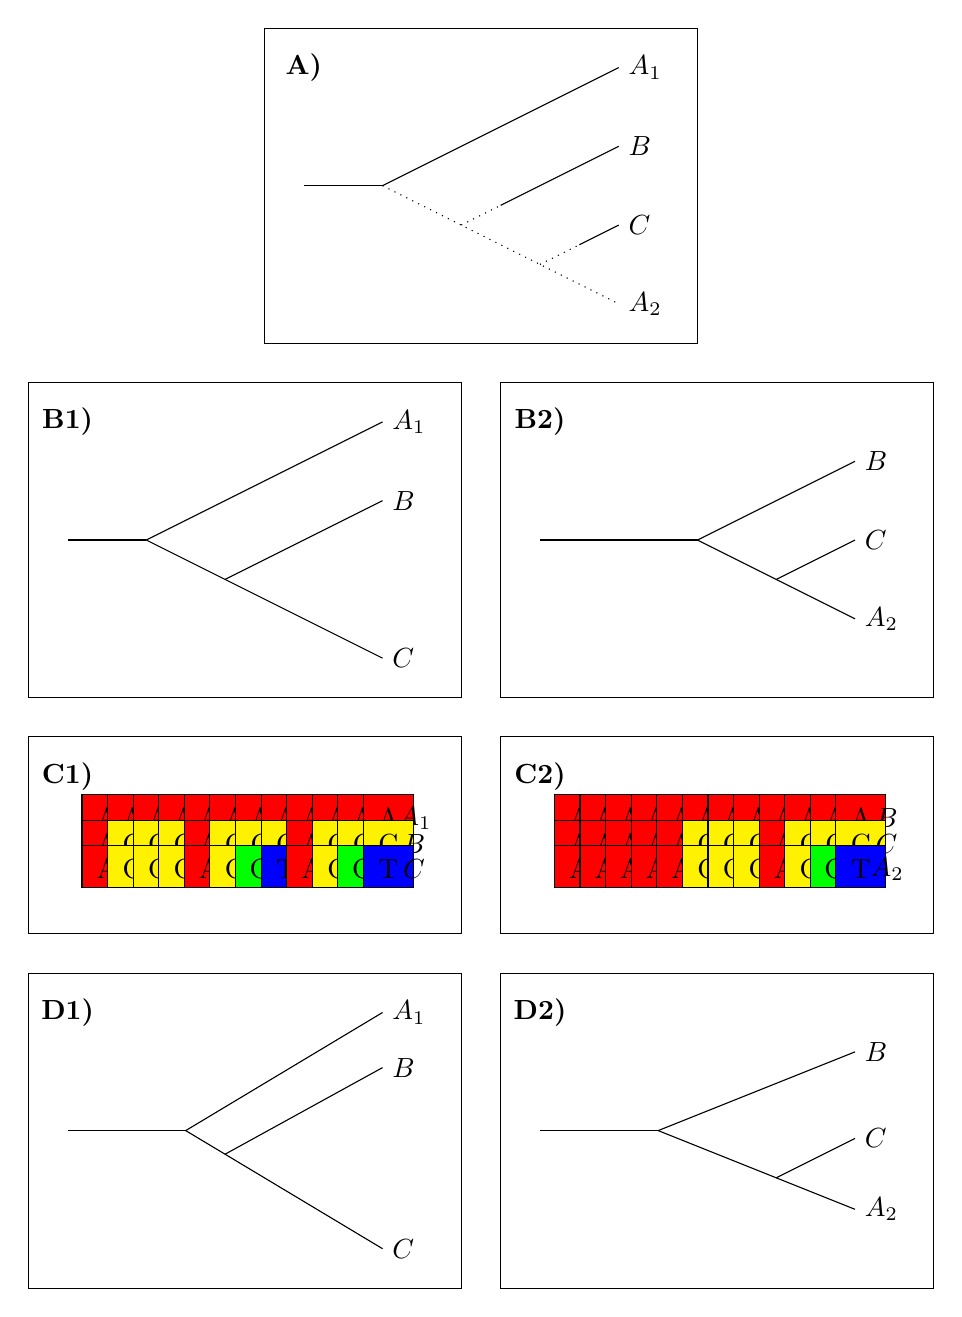
\begin{tikzpicture}[scale = 0.5]

  % Incipient species tree
  \begin{scope}[shift={(0,0)}] 

    \node[font = \bf] at (0, 0) {A)};
    \draw (-1,1) rectangle (10,-7);

    % Drawing of the phylogeny
    \begin{scope}[shift={(0,-3)}] 
      \draw (0, 0) -- (2,  0); % stem 
      \draw (2, 0) -- (8,  3) node[anchor=west] {$A_1$};
      \draw[dotted] (4,  -1) -- (5, -0.5); \draw (5, -0.5) -- (8, 1) node[anchor=west] {$B$};
      \draw[dotted] (6,  -2) -- (7, -1.5); \draw (7, -1.5) -- (8, -1) node[anchor=west] {$C$};
      \draw[dotted] (2,0) -- (8, -3) node[anchor=west] {$A_2$};
    \end{scope} % Drawing of the phylogeny

  \end{scope}


  % Species tree, oldest
  \begin{scope}[shift={(-6,-9)}] 

    \node[font = \bf] at (0.0, 0  ) {B1)};
    \draw (-1,1) rectangle (10,-7);

    % Drawing of the species tree, oldest
    \begin{scope}[shift={(0,-3)}] 
      \draw (0, 0) -- (2,  0); % stem 
      \draw (2, 0) -- (8,  3) node[anchor=west] {$A_1$};
      \draw (4,  -1) -- (8, 1) node[anchor=west] {$B$};
      \draw (2,0) -- (8, -3) node[anchor=west] {$C$};
    \end{scope} % Drawing of the species tree, oldest

  \end{scope}


  % Species tree, youngest
  \begin{scope}[shift={( 6,-9)}] 

    \node[font = \bf] at (0, 0) {B2)};
    \draw (-1,1) rectangle (10,-7);

    % Drawing of the species tree, youngest
    \begin{scope}[shift={(0,-3)}] 
      \draw (0, 0) -- (4,  0); % stem 
      \draw (4, 0) -- (8,  2) node[anchor=west] {$B$};
      \draw (6,-1) -- (8,  0) node[anchor=west] {$C$};
      \draw (4, 0) -- (8, -2) node[anchor=west] {$A_2$};
    \end{scope} % Drawing of the species tree, youngest

  \end{scope}

  % Alignment, oldest
  \begin{scope}[shift={(-6,-18)}] 

    \node[font = \bf] at (0.0, 0  ) {C1)};
    \draw (-1,1) rectangle (10,-4);

    % Drawing of the alignment
    \begin{scope}[shift={(1,-1)}, text width = 4mm, text height = 3mm, align = center, scale = 1.3] 

      \node[draw, fill = red   ] at (0.0, 0  ) {A};
      \node[draw, fill = red   ] at (0.5, 0  ) {A};
      \node[draw, fill = red   ] at (1.0, 0  ) {A};
      \node[draw, fill = red   ] at (1.5, 0  ) {A};
      \node[draw, fill = red   ] at (2.0, 0  ) {A};
      \node[draw, fill = red   ] at (2.5, 0  ) {A};
      \node[draw, fill = red   ] at (3.0, 0  ) {A};
      \node[draw, fill = red   ] at (3.5, 0  ) {A};
      \node[draw, fill = red   ] at (4.0, 0  ) {A};
      \node[draw, fill = red   ] at (4.5, 0  ) {A};
      \node[draw, fill = red   ] at (5.0, 0  ) {A};
      \node[draw, fill = red   ] at (5.5, 0  ) {A};
      \node[                   ] at (6.0, 0  ) {$A_1$};

      \node[draw, fill = red   ] at (0.0, -0.5) {A};
      \node[draw, fill = yellow] at (0.5, -0.5) {C};
      \node[draw, fill = yellow] at (1.0, -0.5) {C};
      \node[draw, fill = yellow] at (1.5, -0.5) {C};
      \node[draw, fill = red   ] at (2.0, -0.5) {A};
      \node[draw, fill = yellow] at (2.5, -0.5) {C};
      \node[draw, fill = yellow] at (3.0, -0.5) {C};
      \node[draw, fill = yellow] at (3.5, -0.5) {C};
      \node[draw, fill = red   ] at (4.0, -0.5) {A};
      \node[draw, fill = yellow] at (4.5, -0.5) {C};
      \node[draw, fill = yellow] at (5.0, -0.5) {C};
      \node[draw, fill = yellow] at (5.5, -0.5) {C};
      \node[                   ] at (6.0, -0.5) {$B$};

      \node[draw, fill = red] at (0.0, -1.0) {A};
      \node[draw, fill = yellow] at (0.5, -1.0) {C};
      \node[draw, fill = yellow] at (1.0, -1.0) {C};
      \node[draw, fill = yellow] at (1.5, -1.0) {C};
      \node[draw, fill = red   ] at (2.0, -1.0) {A};
      \node[draw, fill = yellow] at (2.5, -1.0) {C};
      \node[draw, fill = green ] at (3.0, -1.0) {G};
      \node[draw, fill = blue  ] at (3.5, -1.0) {T};
      \node[draw, fill = red   ] at (4.0, -1.0) {A};
      \node[draw, fill = yellow] at (4.5, -1.0) {C};
      \node[draw, fill = green ] at (5.0, -1.0) {G};
      \node[draw, fill = blue  ] at (5.5, -1.0) {T};
      \node[                   ] at (6.0, -1.0) {$C$};

    \end{scope} % Drawing of the alignment

  \end{scope}

  % Alignment, youngest
  \begin{scope}[shift={(6,-18)}] 

    \node[font = \bf] at (0.0, 0  ) {C2)};
    \draw (-1,1) rectangle (10,-4);

    % Drawing of the alignment
    \begin{scope}[shift={(1,-1)}, text width = 4mm, text height = 3mm, align = center, scale = 1.3] 

      \node[draw, fill = red   ] at (0.0, 0  ) {A};
      \node[draw, fill = red   ] at (0.5, 0  ) {A};
      \node[draw, fill = red   ] at (1.0, 0  ) {A};
      \node[draw, fill = red   ] at (1.5, 0  ) {A};
      \node[draw, fill = red   ] at (2.0, 0  ) {A};
      \node[draw, fill = red   ] at (2.5, 0  ) {A};
      \node[draw, fill = red   ] at (3.0, 0  ) {A};
      \node[draw, fill = red   ] at (3.5, 0  ) {A};
      \node[draw, fill = red   ] at (4.0, 0  ) {A};
      \node[draw, fill = red   ] at (4.5, 0  ) {A};
      \node[draw, fill = red   ] at (5.0, 0  ) {A};
      \node[draw, fill = red   ] at (5.5, 0  ) {A};
      \node[                   ] at (6.0, 0  ) {$B$};

      \node[draw, fill = red   ] at (0.0, -0.5) {A};
      \node[draw, fill = red   ] at (0.5, -0.5) {A};
      \node[draw, fill = red   ] at (1.0, -0.5) {A};
      \node[draw, fill = red   ] at (1.5, -0.5) {A};
      \node[draw, fill = red   ] at (2.0, -0.5) {A};
      \node[draw, fill = yellow] at (2.5, -0.5) {C};
      \node[draw, fill = yellow] at (3.0, -0.5) {C};
      \node[draw, fill = yellow] at (3.5, -0.5) {C};
      \node[draw, fill = red   ] at (4.0, -0.5) {A};
      \node[draw, fill = yellow] at (4.5, -0.5) {C};
      \node[draw, fill = yellow] at (5.0, -0.5) {C};
      \node[draw, fill = yellow] at (5.5, -0.5) {C};
      \node[                   ] at (6.0, -0.5) {$C$};

      \node[draw, fill = red   ] at (0.0, -1.0) {A};
      \node[draw, fill = red   ] at (0.5, -1.0) {A};
      \node[draw, fill = red   ] at (1.0, -1.0) {A};
      \node[draw, fill = red   ] at (1.5, -1.0) {A};
      \node[draw, fill = red   ] at (2.0, -1.0) {A};
      \node[draw, fill = yellow] at (2.5, -1.0) {C};
      \node[draw, fill = yellow] at (3.0, -1.0) {C};
      \node[draw, fill = yellow] at (3.5, -1.0) {C};
      \node[draw, fill = red   ] at (4.0, -1.0) {A};
      \node[draw, fill = yellow] at (4.5, -1.0) {C};
      \node[draw, fill = green ] at (5.0, -1.0) {G};
      \node[draw, fill = blue  ] at (5.5, -1.0) {T};
      \node[                   ] at (6.0, -1.0) {$A_2$};

    \end{scope} % Drawing of the alignment

  \end{scope}



  % Estimated species tree, oldest
  \begin{scope}[shift={(-6,-24)}] 

    \node[font = \bf] at (0, 0) {D1)};
    \draw (-1,1) rectangle (10,-7);

    \begin{scope}[shift={(0,-3)}] 
      \draw (0, 0) -- (3,  0);
      \draw (3, 0) -- (8, 3) node[anchor=west] {$A_1$};
      \draw (4,-0.6) -- (8, 1.6) node[anchor=west] {$B$};
      \draw (3, 0) -- (8,-3) node[anchor=west] {$C$};
    \end{scope}

  \end{scope}


  % Estimated species tree, youngest
  \begin{scope}[shift={(6,-24)}] 

    \node[font = \bf] at (0, 0) {D2)};
    \draw (-1,1) rectangle (10,-7);

    \begin{scope}[shift={(0,-3)}] 
      \draw (0, 0) -- (3,  0);
      \draw (3, 0) -- (8,  2) node[anchor=west] {$B$};
      \draw (6,-1.2) -- (8, -0.2) node[anchor=west] {$C$};
      \draw (3, 0) -- (8, -2) node[anchor=west] {$A_2$};
    \end{scope}

  \end{scope}

\end{tikzpicture}
%%%%%%%%%%%%%%%%%%%%%%%%%%%%%%%%%%%%%%%%%%%%%%%%%%%%%%%%%%%%%%%%%%%%%%%%%%%%%%%%




%%%%%%%%%%%%%%%%%%%%%%%%%%%%%%%%%%%%%%%%%%%%%%%%%%%%%%%%%%%%%%%%%%%%%%%%%%%%%%%%
% Create the TikZ picture of fig:sampling
%%%%%%%%%%%%%%%%%%%%%%%%%%%%%%%%%%%%%%%%%%%%%%%%%%%%%%%%%%%%%%%%%%%%%%%%%%%%%%%%
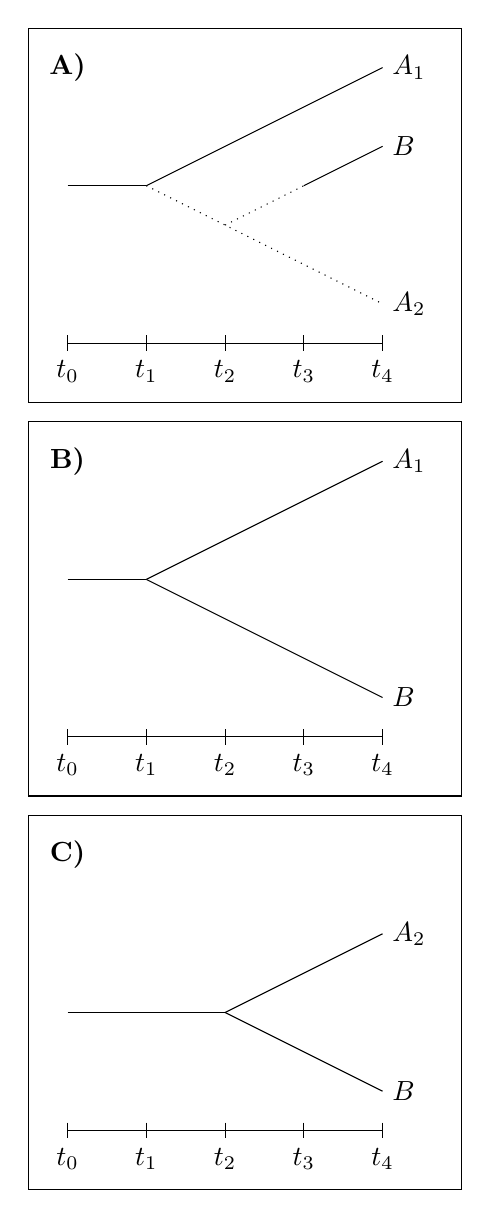
\begin{tikzpicture}[scale = 0.5] 

  \begin{scope}[shift={(0,0)}] 

    \node[font = \bf] at (0, 0) {A)};
    \draw (-1,1) rectangle (10,-8.5);

    % Drawing of the phylogeny
    \begin{scope}[shift={(0,-3)}] 
      \draw (0, 0) -- (2,  0);
      \draw (2, 0) -- (8,  3) node[anchor=west] {$A_1$};
      \draw[dotted] (2, 0) -- (8, -3) node[anchor=west] {$A_2$};
      \draw[dotted] (4, -1) -- (6, 0);
      \draw (6, 0) -- (8, 1) node[anchor=west] {$B$};
      % time scale
      \draw (0, -4) -- (8,  -4);
      \draw (0, -3.8) -- (0,  -4.2) node[anchor=north] {$t_0$};
      \draw (2, -3.8) -- (2,  -4.2) node[anchor=north] {$t_1$};
      \draw (4, -3.8) -- (4,  -4.2) node[anchor=north] {$t_2$};
      \draw (6, -3.8) -- (6,  -4.2) node[anchor=north] {$t_3$};
      \draw (8, -3.8) -- (8,  -4.2) node[anchor=north] {$t_4$};
    \end{scope} % Drawing of the phylogeny

  \end{scope}
  \begin{scope}[shift={(0, -10)}] 

    \node[font = \bf] at (0, 0) {B)};
    \draw (-1,1) rectangle (10,-8.5);

    % Drawing of the phylogeny
    \begin{scope}[shift={(0,-3)}] 
      \draw (0, 0) -- (2,  0);
      \draw (2, 0) -- (8,  3) node[anchor=west] {$A_1$};
      \draw (2, 0) -- (8, -3) node[anchor=west] {$B$};
      % time scale
      \draw (0, -4) -- (8,  -4);
      \draw (0, -3.8) -- (0,  -4.2) node[anchor=north] {$t_0$};
      \draw (2, -3.8) -- (2,  -4.2) node[anchor=north] {$t_1$};
      \draw (4, -3.8) -- (4,  -4.2) node[anchor=north] {$t_2$};
      \draw (6, -3.8) -- (6,  -4.2) node[anchor=north] {$t_3$};
      \draw (8, -3.8) -- (8,  -4.2) node[anchor=north] {$t_4$};
    \end{scope} % Drawing of the phylogeny

  \end{scope}
  \begin{scope}[shift={(0,-20)}] 

    \node[font = \bf] at (0, 0) {C)};
    \draw (-1,1) rectangle (10,-8.5);

    % Drawing of the phylogeny
    \begin{scope}[shift={(0,-3)}] 
      \draw (0, -1) -- (4, -1) ;
      \draw (4, -1) -- (8, -3) node[anchor=west] {$B$};
      \draw (4, -1) -- (8,  1) node[anchor=west] {$A_2$};
      % time scale
      \draw (0, -4) -- (8,  -4);
      \draw (0, -3.8) -- (0,  -4.2) node[anchor=north] {$t_0$};
      \draw (2, -3.8) -- (2,  -4.2) node[anchor=north] {$t_1$};
      \draw (4, -3.8) -- (4,  -4.2) node[anchor=north] {$t_2$};
      \draw (6, -3.8) -- (6,  -4.2) node[anchor=north] {$t_3$};
      \draw (8, -3.8) -- (8,  -4.2) node[anchor=north] {$t_4$};
    \end{scope} % Drawing of the phylogeny

  \end{scope}
\end{tikzpicture}
%%%%%%%%%%%%%%%%%%%%%%%%%%%%%%%%%%%%%%%%%%%%%%%%%%%%%%%%%%%%%%%%%%%%%%%%%%%%%%%%

\end{document}
